\documentclass[../main.tex]{subfiles}
% DOCUMENT

\begin{document}

\section{Trường hợp thực tế}\label{case-study}

Ngoài việc thử nghiệm với các dữ liệu sinh ngẫu nhiên, thuật toán DDD cho bài toán MDP đã được thử  
nghiệm trên bộ dữ liệu thực tế từ mạng lưới
đường bộ Atlanta (\cite{he2022dynamic}). Mạng này bao gồm 306 nút và 618 cung, được lấy từ Open
Street Map. \autoref{fig:14} mô tả bản đồ khu vực và biểu diễn mạng lưới tương
ứng.

% \begin{figure}
% \centering
% 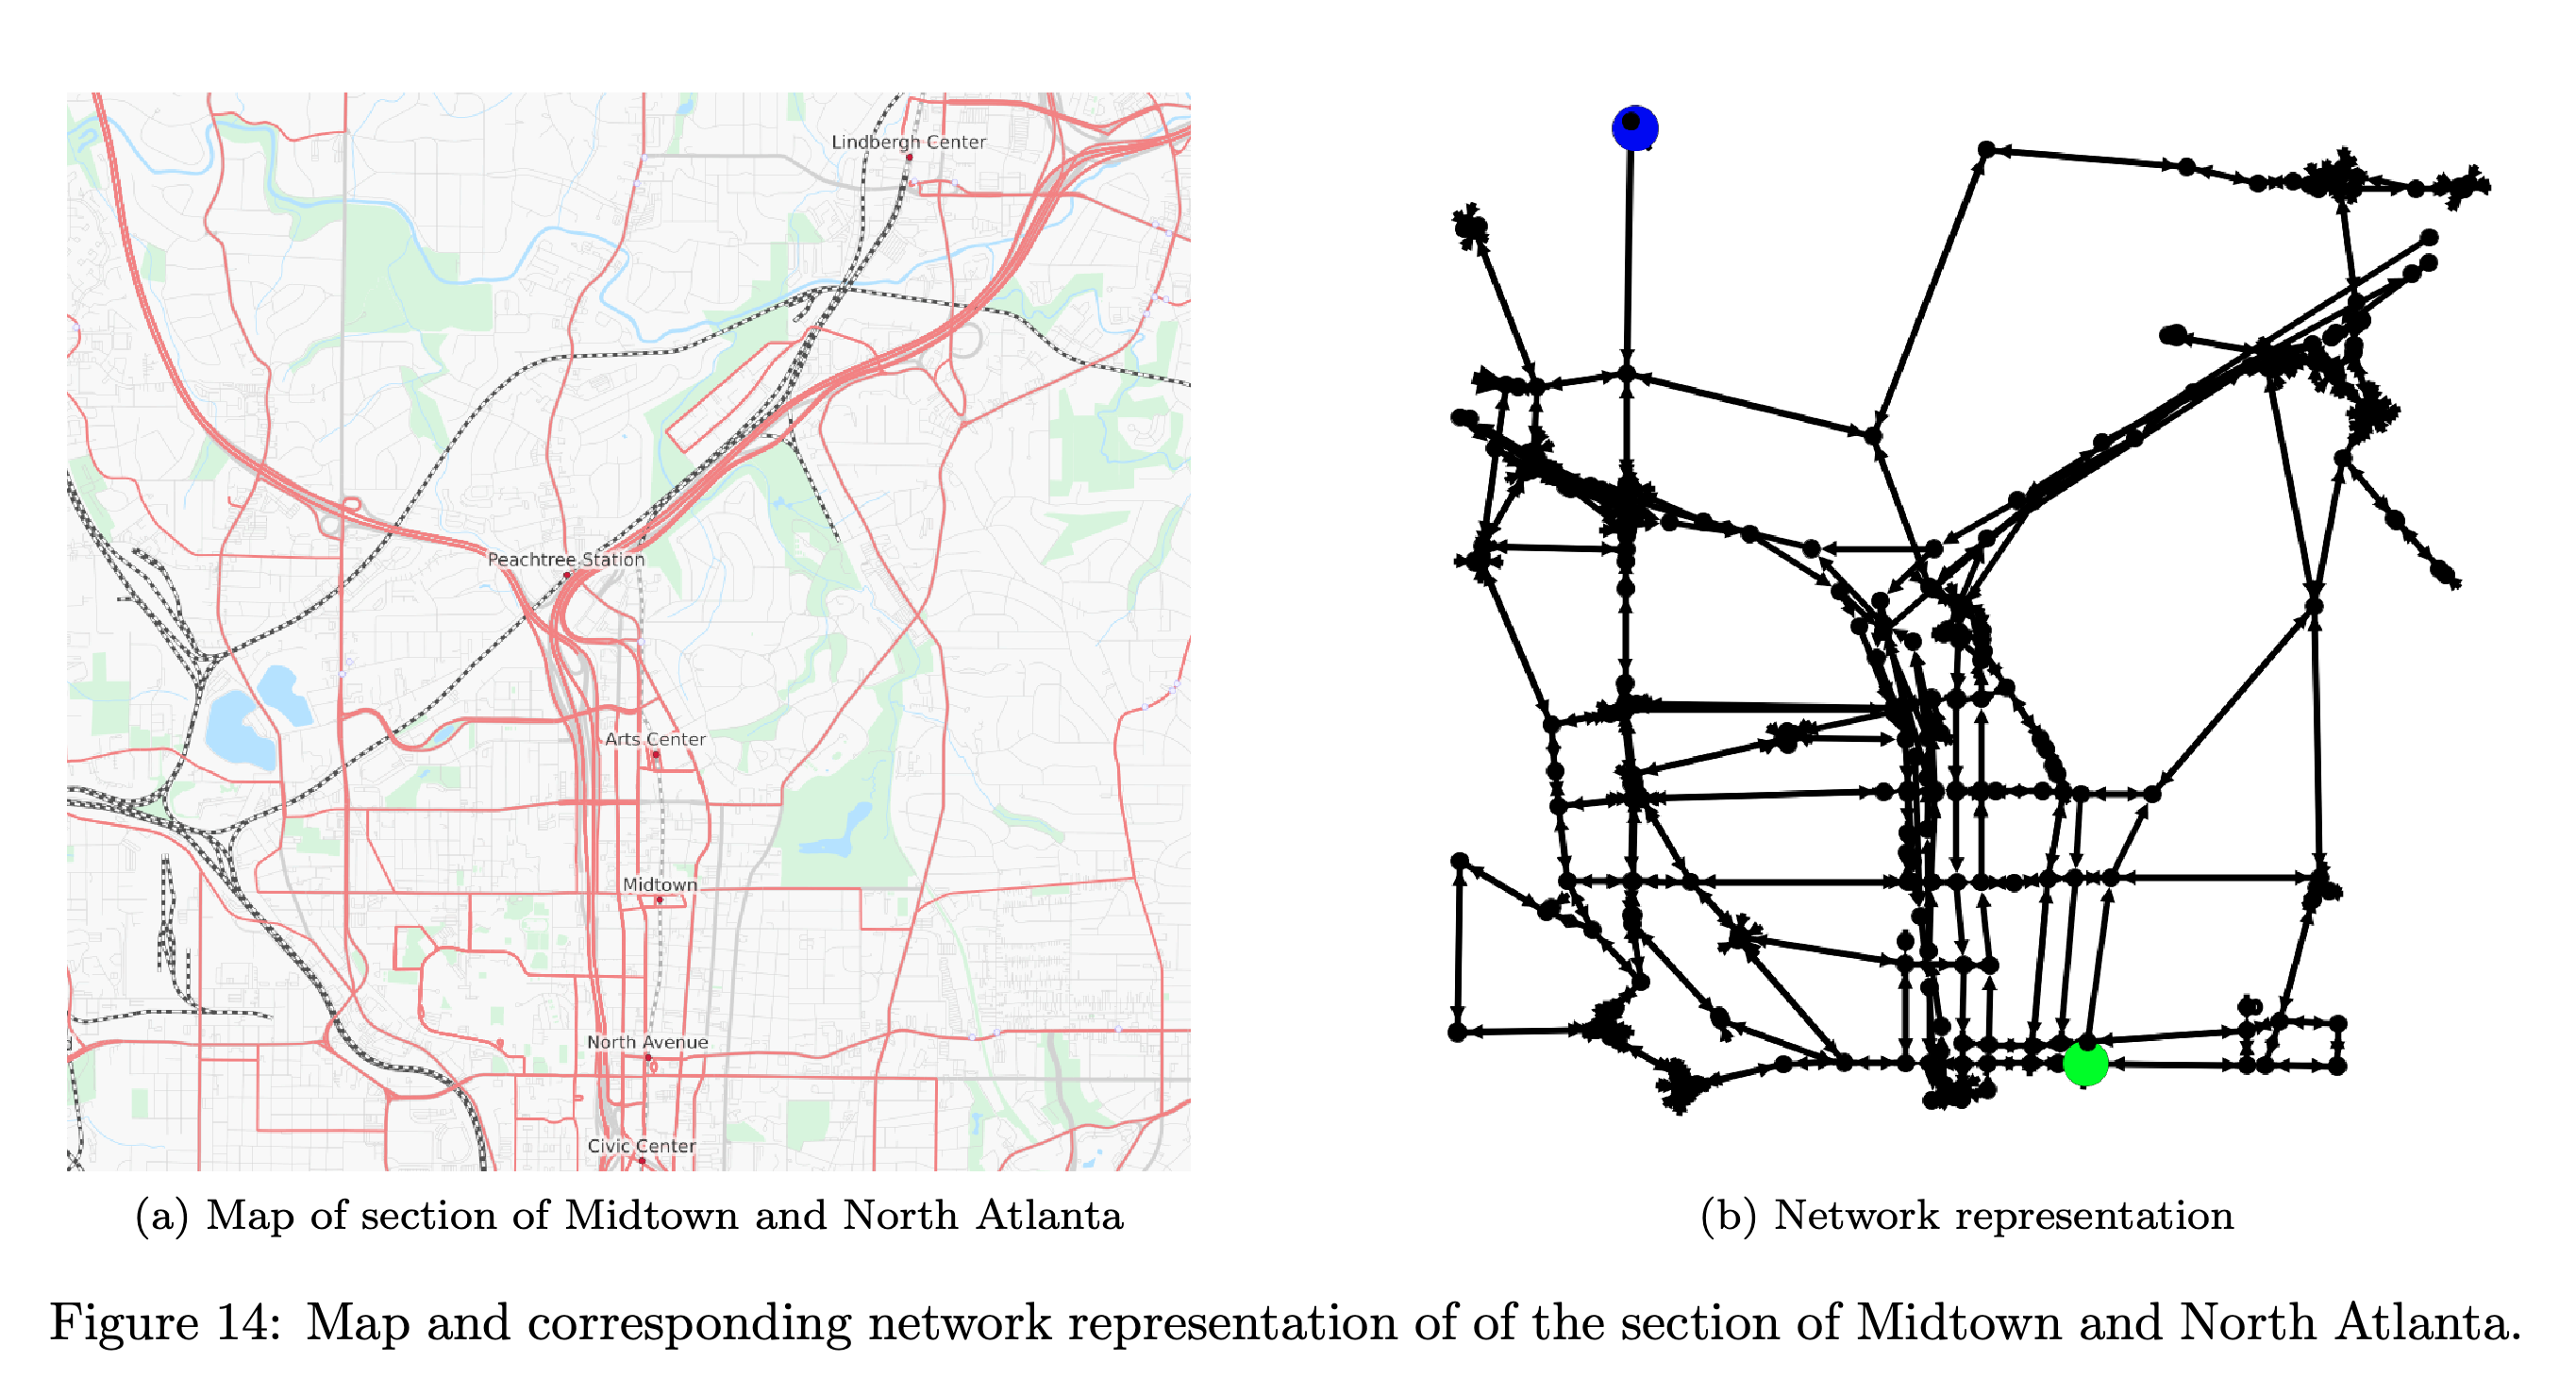
\includegraphics{images/Figure14.png}
% \caption{Figure14}
% \label{fig:14}
% \end{figure}

\begin{figure}
    \centering
    \begin{subfigure}{0.45\textwidth}
        \centering
        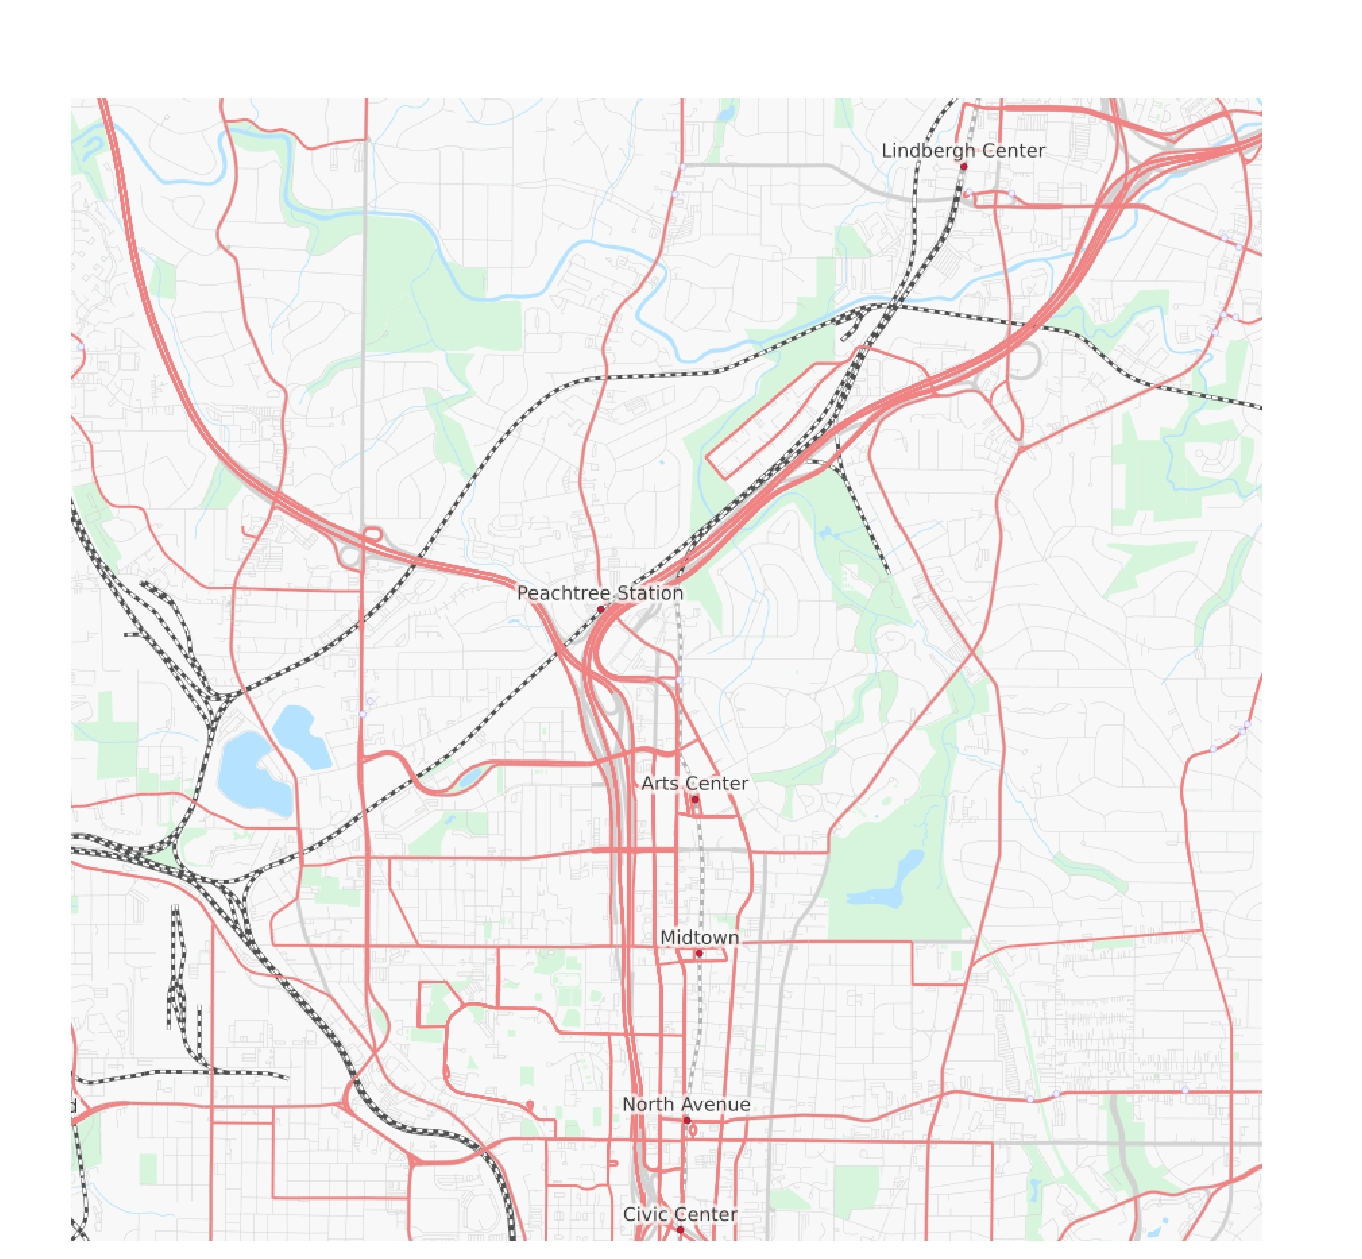
\includegraphics{edited-images/Figure14a.jpg}
        \caption{Bản đồ khu vực}
        \label{fig:14a}
    \end{subfigure}
    \begin{subfigure}{0.45\textwidth}
        \centering
        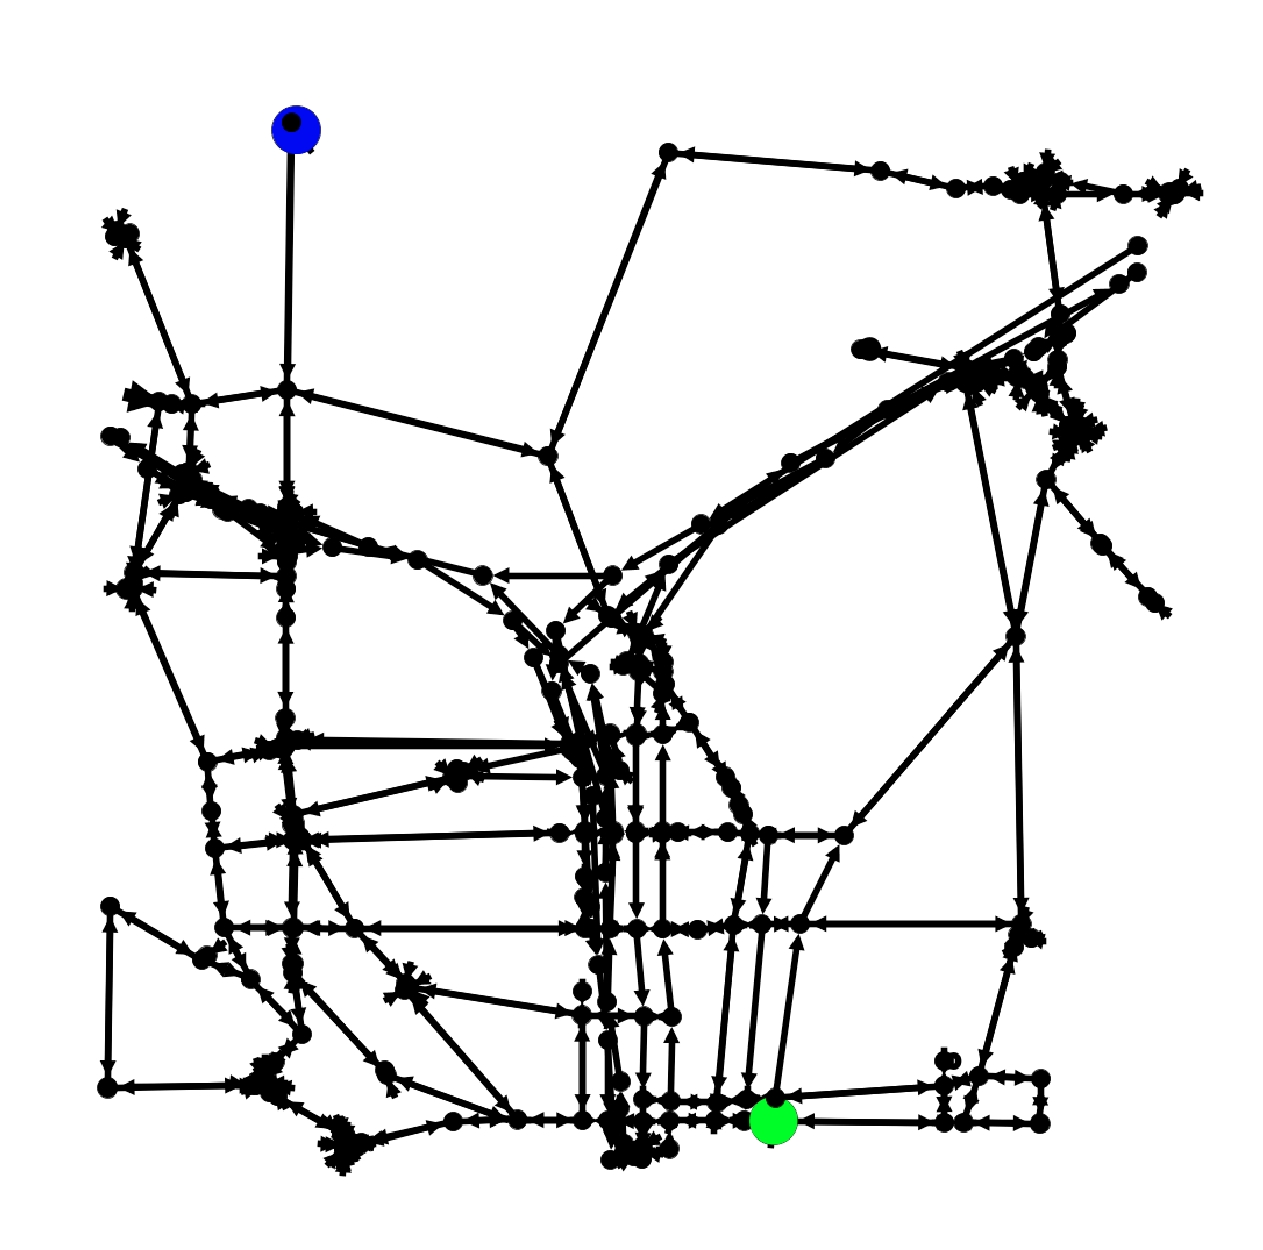
\includegraphics{edited-images/Figure14b.jpg}
        \caption{Mạng lưới đường bộ}
        \label{fig:14b}
    \end{subfigure}
    \caption{Bản đồ và mạng lưới đường bộ khu vực Trung tâm và phía Bắc Atlanta}
    \label{fig:14}
\end{figure}

Dữ liệu về thời gian di chuyển được thu thập từ nhiều nguồn khác nhau
(hệ thống định vị, dữ liệu di động). Dữ liệu được thu thập và tổng hợp
để tạo thành các hàm vận tốc tuyến tính từng khúc với các BP
cách nhau 15 phút trong 24 giờ. Nhờ vậy mỗi cung có tổng cộng 192 điểm
dữ liệu. \autoref{fig:15} là ví dụ về các hàm vận tốc
này.


Để minh họa sự khác biệt giữa đường đi tối thiểu thời gian thực hiện,
đến đích sớm nhất và khởi hành muộn nhất từ nguồn đến đích trong khoảng
thời gian cụ thể, tôi chọn điểm nguồn ở Bắc Atlanta, đích đến ở Trung
tâm Atlanta và khung thời gian là \([9:30, 13:00]\).


Đường đi đến đích sớm nhất mất \(47.5\) phút còn đường đi xuất
phát muộn nhất mất \(47.8\) phút (\autoref{fig:16}). Hai đường đi này đi đường qua đường 
tránh cao tốc, qua khu dân cư (đường Peachtree và đường Juniper) và phải đi đường vòng
để tránh một chiều.

Mặc dù sự khác biệt trong thử nghiệm này không quá lớn (do khu vực
Atlanta được chọn khá bé và ít trường học), việc tìm đường đi chỉ mất
vài giây thời gian chạy. Điều này cho thấy phương pháp này có thể hữu
ích trong thực tế.

% \begin{figure}
% \centering
% 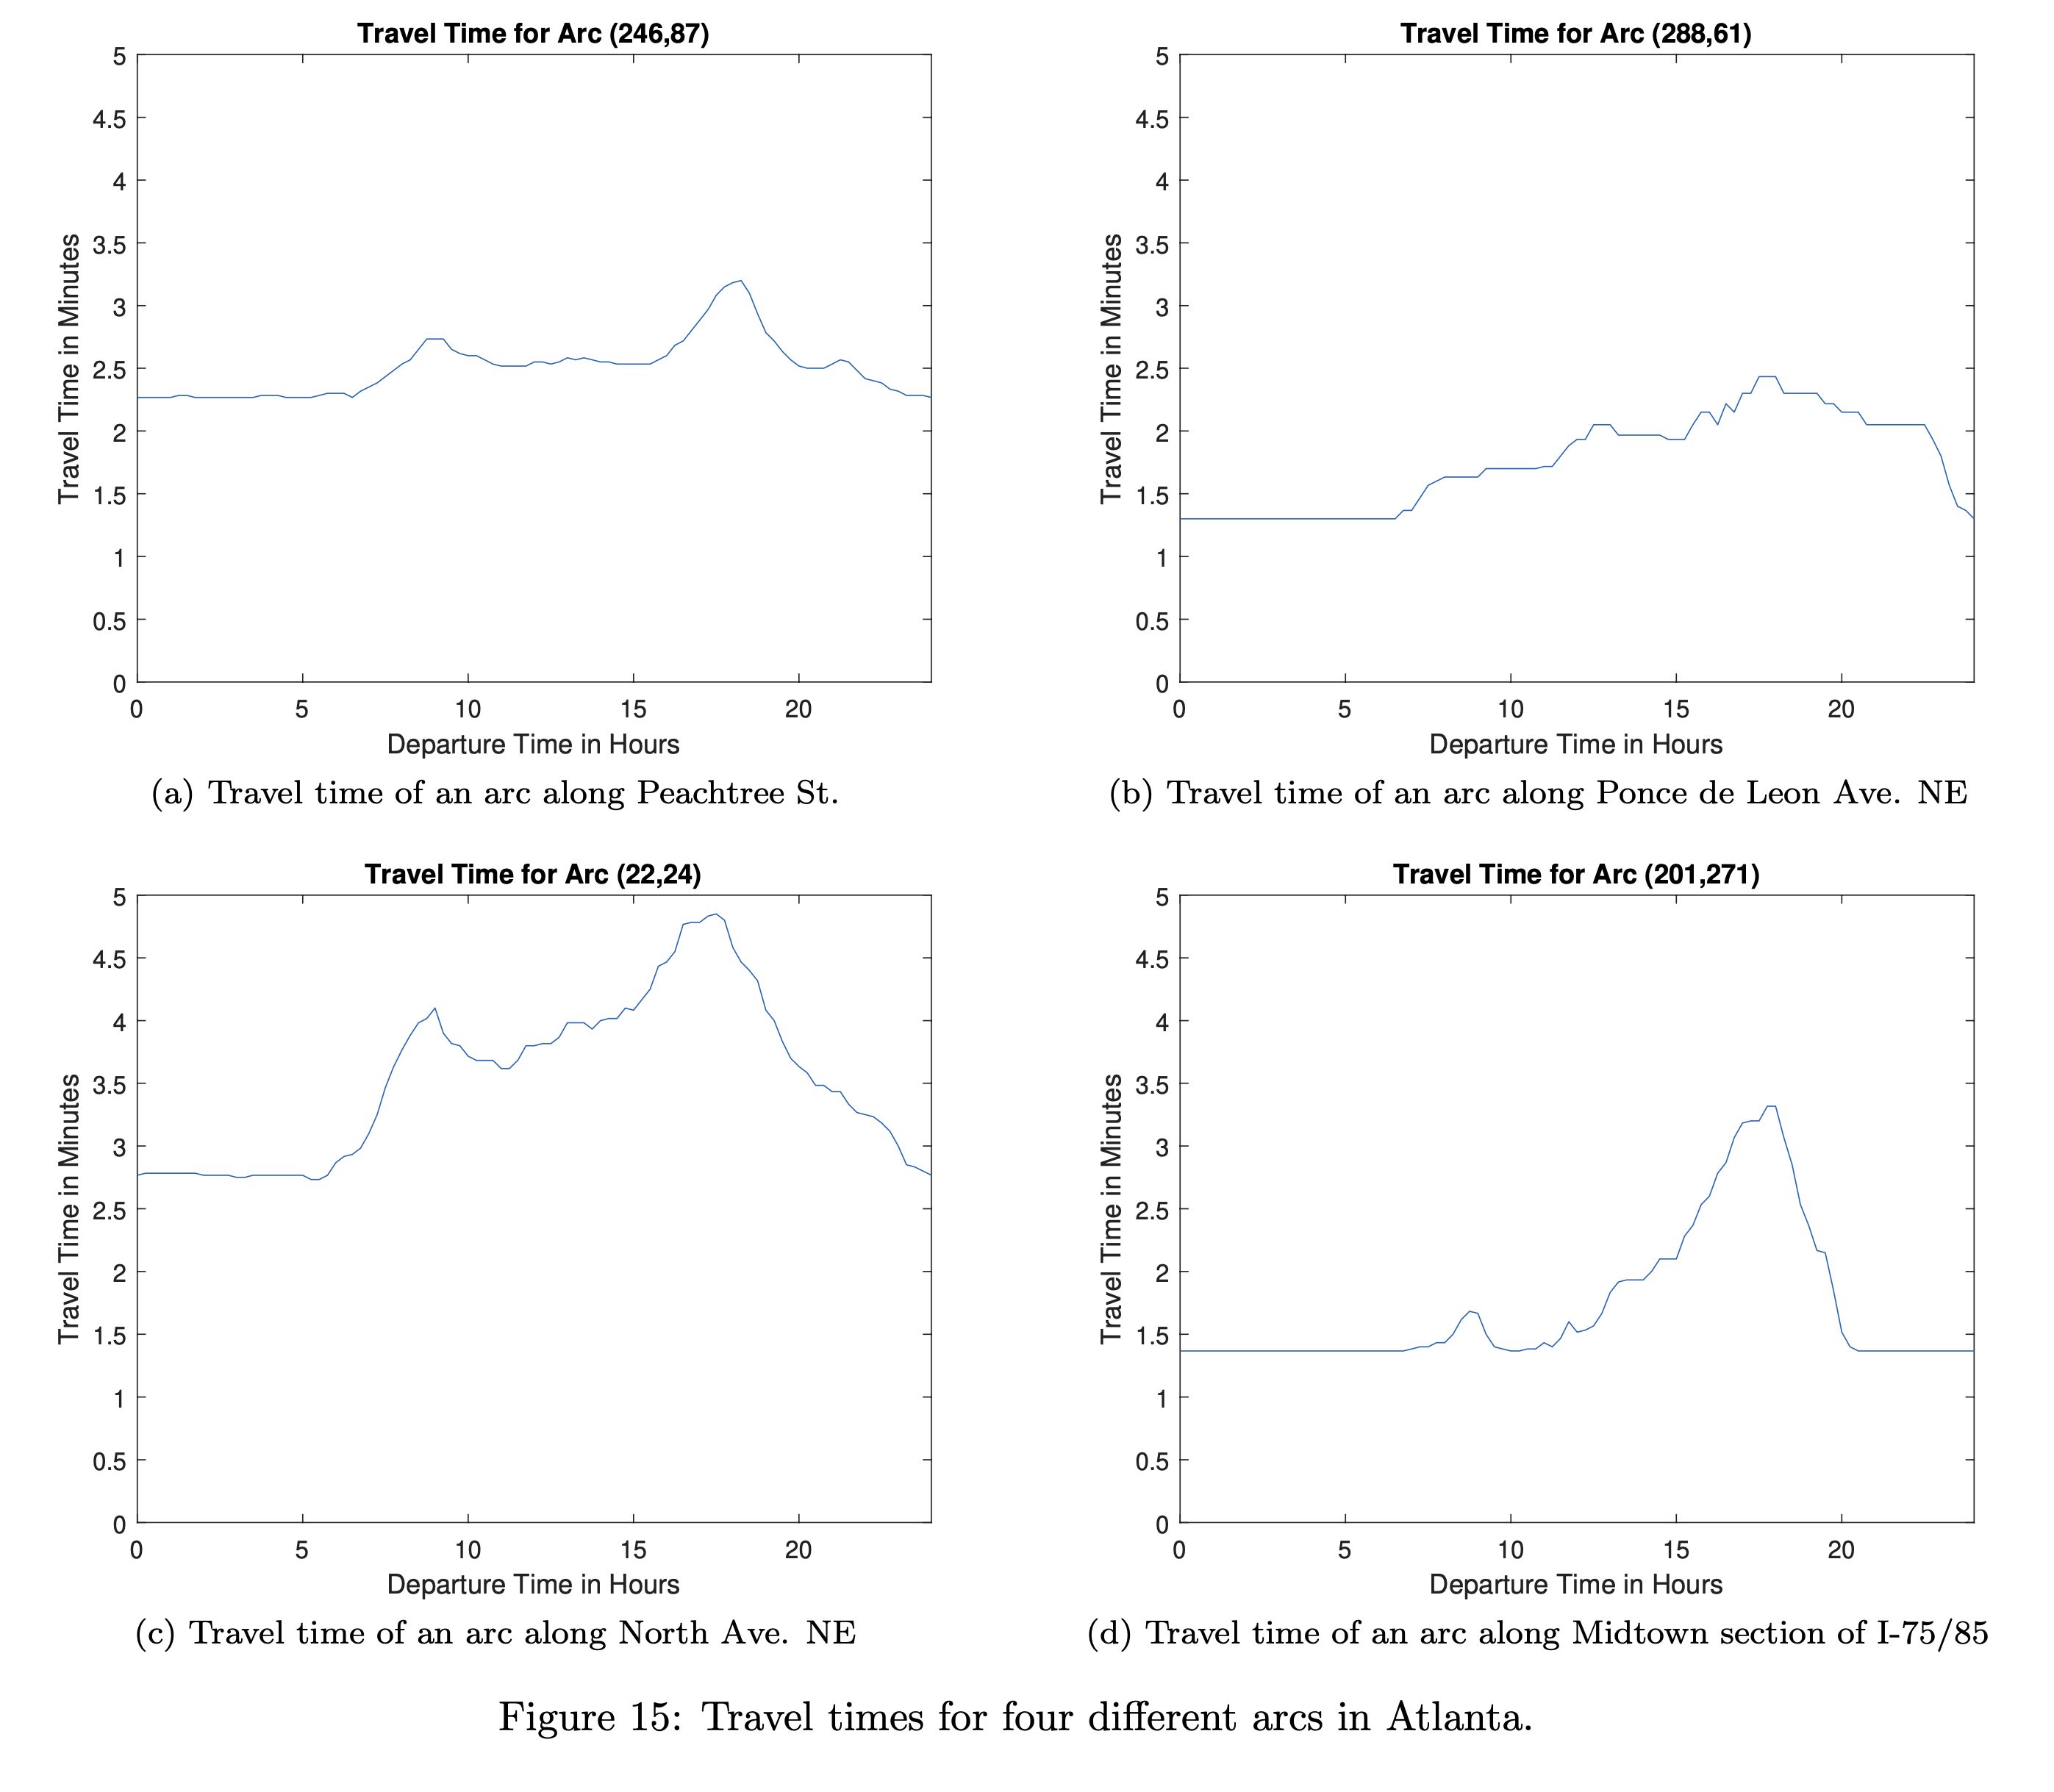
\includegraphics{images/Figure15.png}
% \caption{Figure15}
% \label{fig:15}
% \end{figure}

\begin{figure}
    \centering
    \begin{subfigure}{0.45\textwidth}
        \centering
        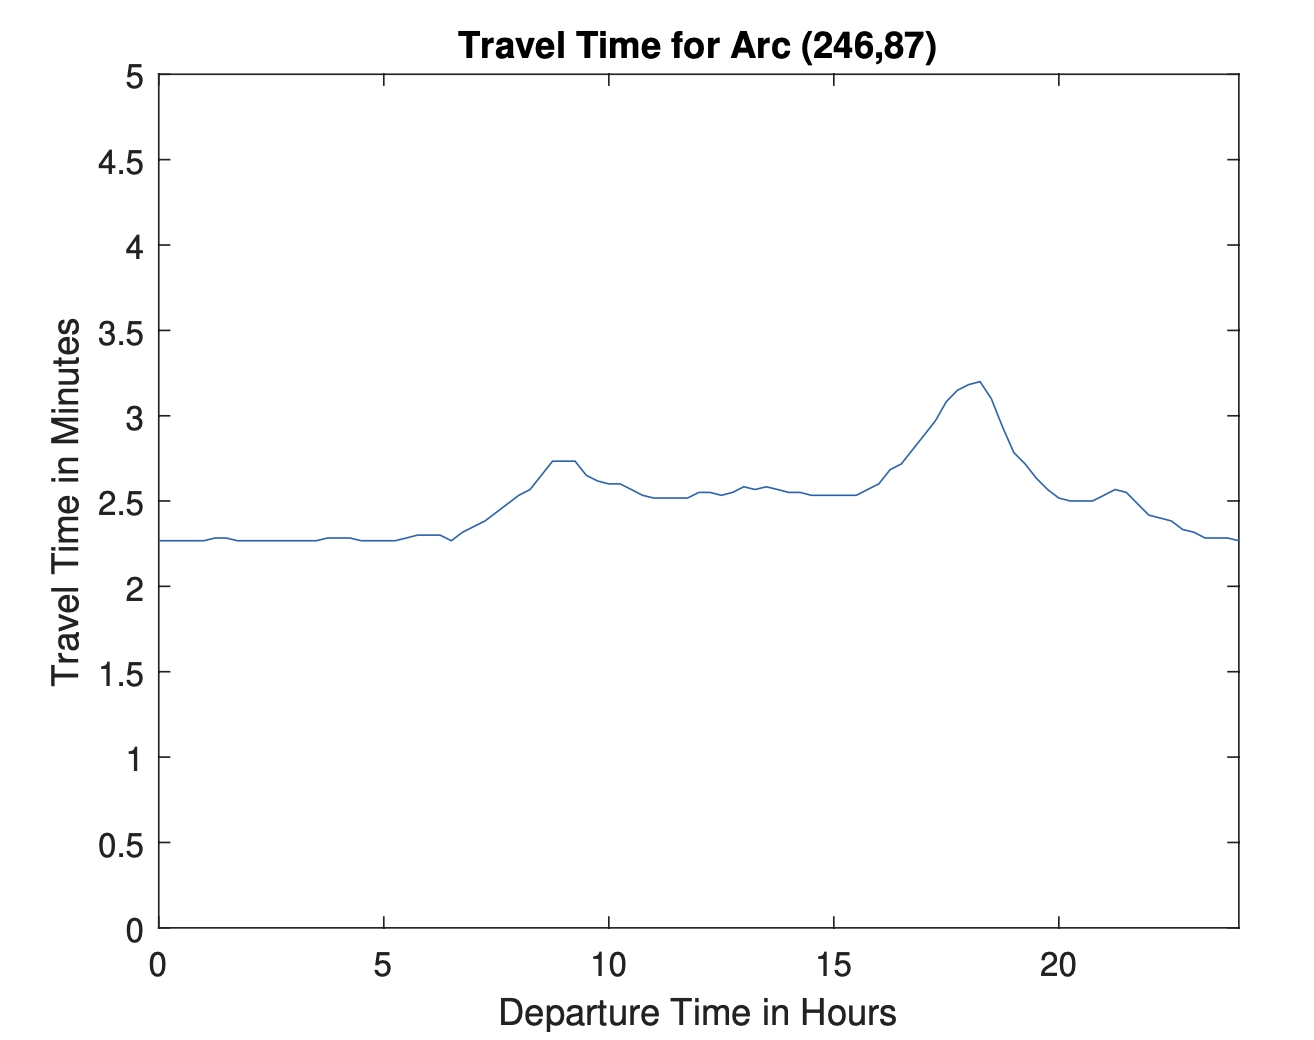
\includegraphics{edited-images/Figure15a.jpg}
        \caption{Đường Peachtree}
        \label{fig:15a}
    \end{subfigure}
    \begin{subfigure}{0.45\textwidth}
        \centering
        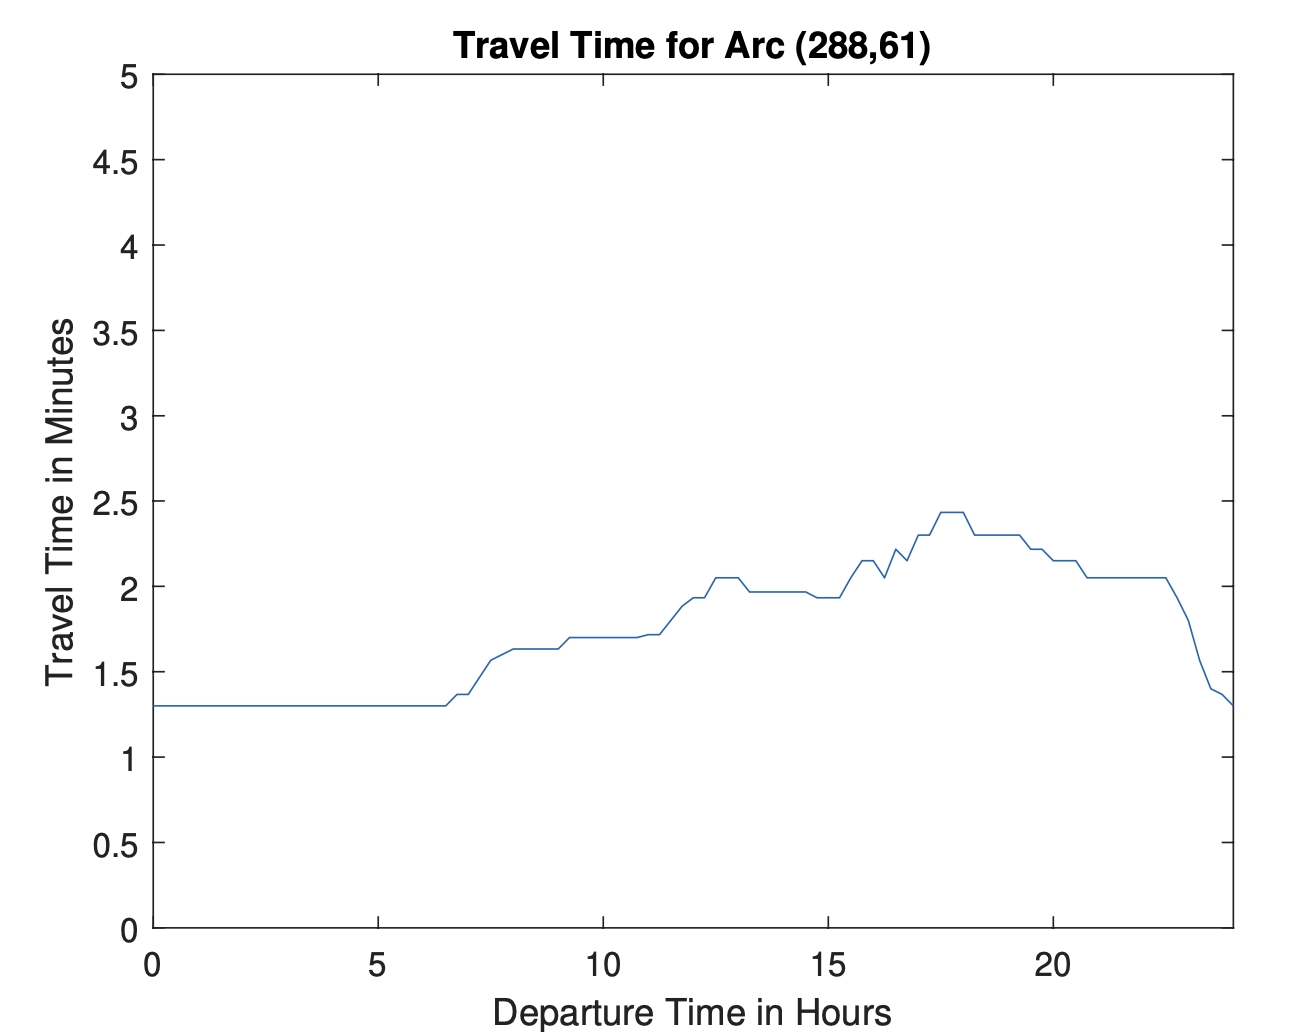
\includegraphics{edited-images/Figure15b.jpg}
        \caption{Đại lộ Ponce de Leon NE}
        \label{fig:15b}
    \end{subfigure}
    \begin{subfigure}{0.45\textwidth}
        \centering
        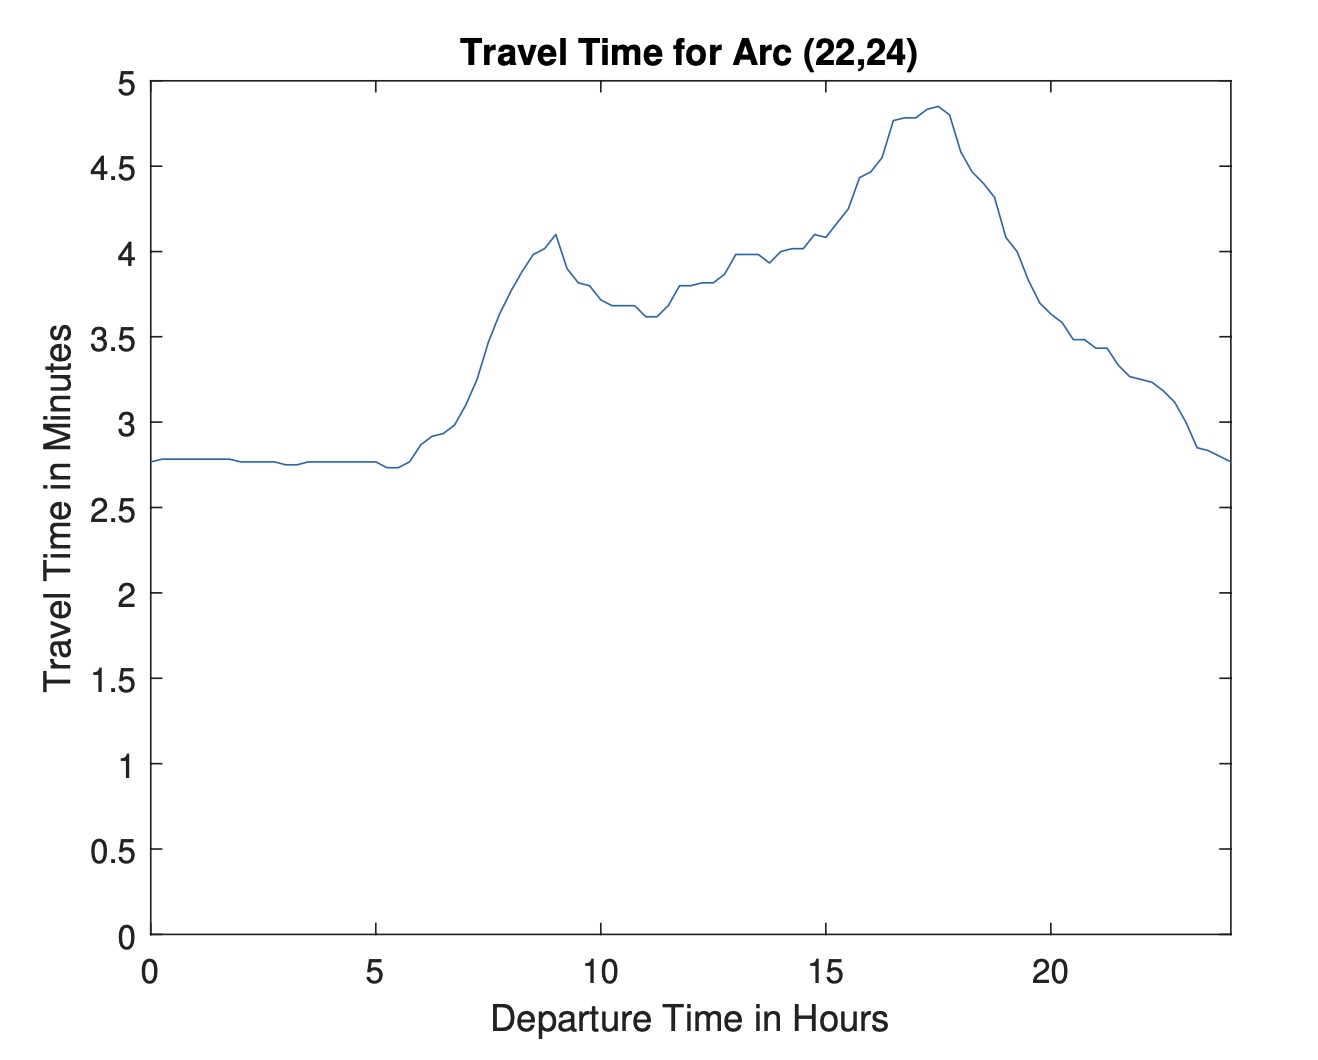
\includegraphics{edited-images/Figure15c.jpg}
        \caption{Bắc Ave. NE}
        \label{fig:15c}
    \end{subfigure}
    \begin{subfigure}{0.45\textwidth}
        \centering
        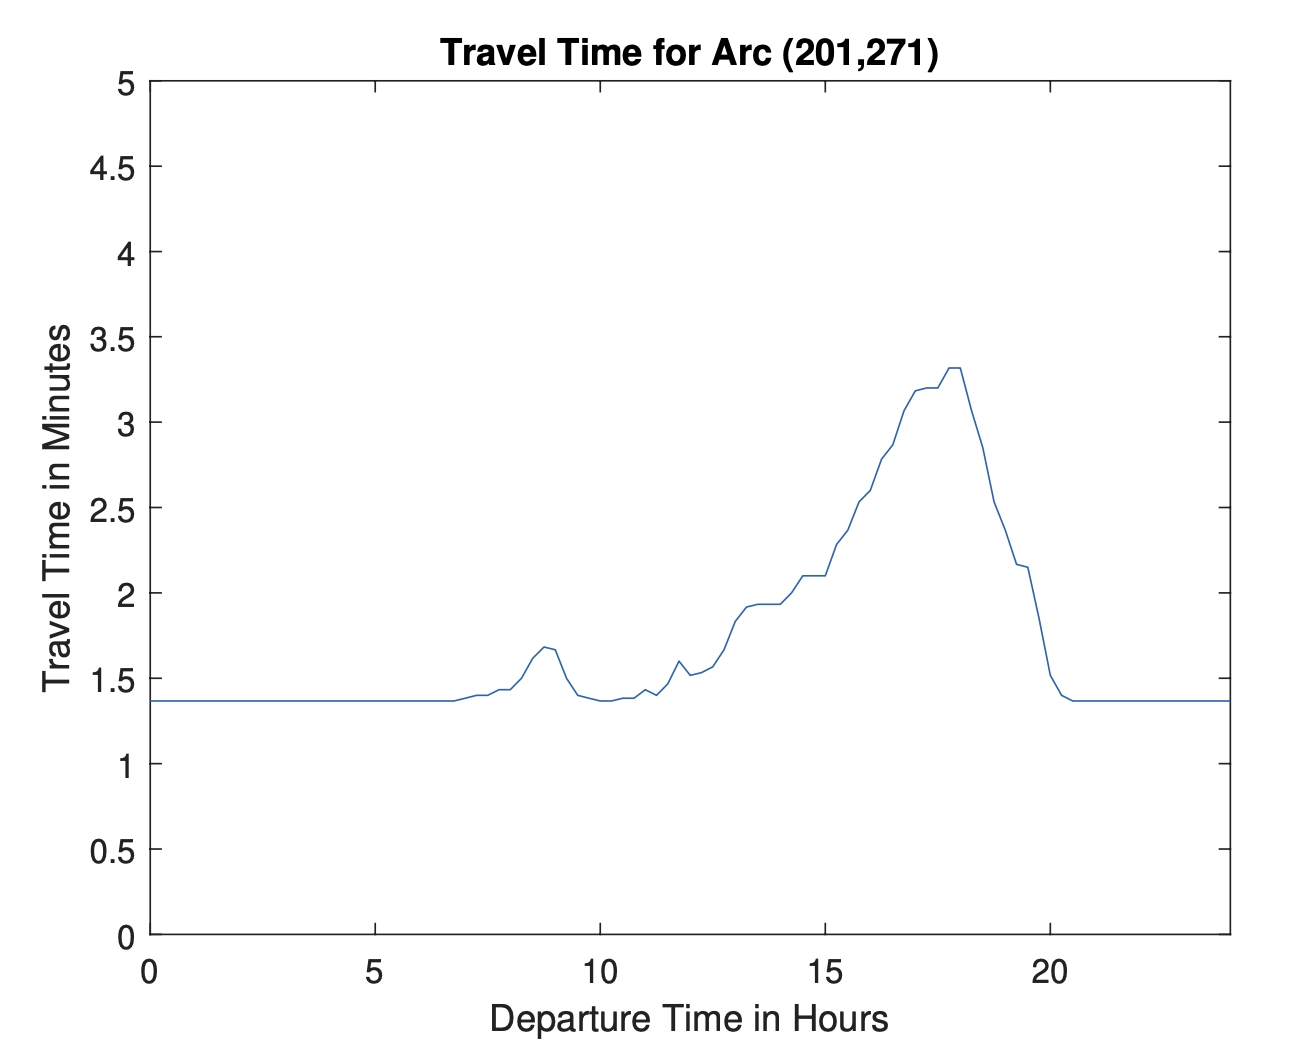
\includegraphics{edited-images/Figure15d.jpg}
        \caption{Trung tâm khu vực I-75/85}
        \label{fig:15d}
    \end{subfigure}
    \caption{Hàm vận tốc các khu vực ở Atlanta}
    \label{fig:15}
\end{figure}

% 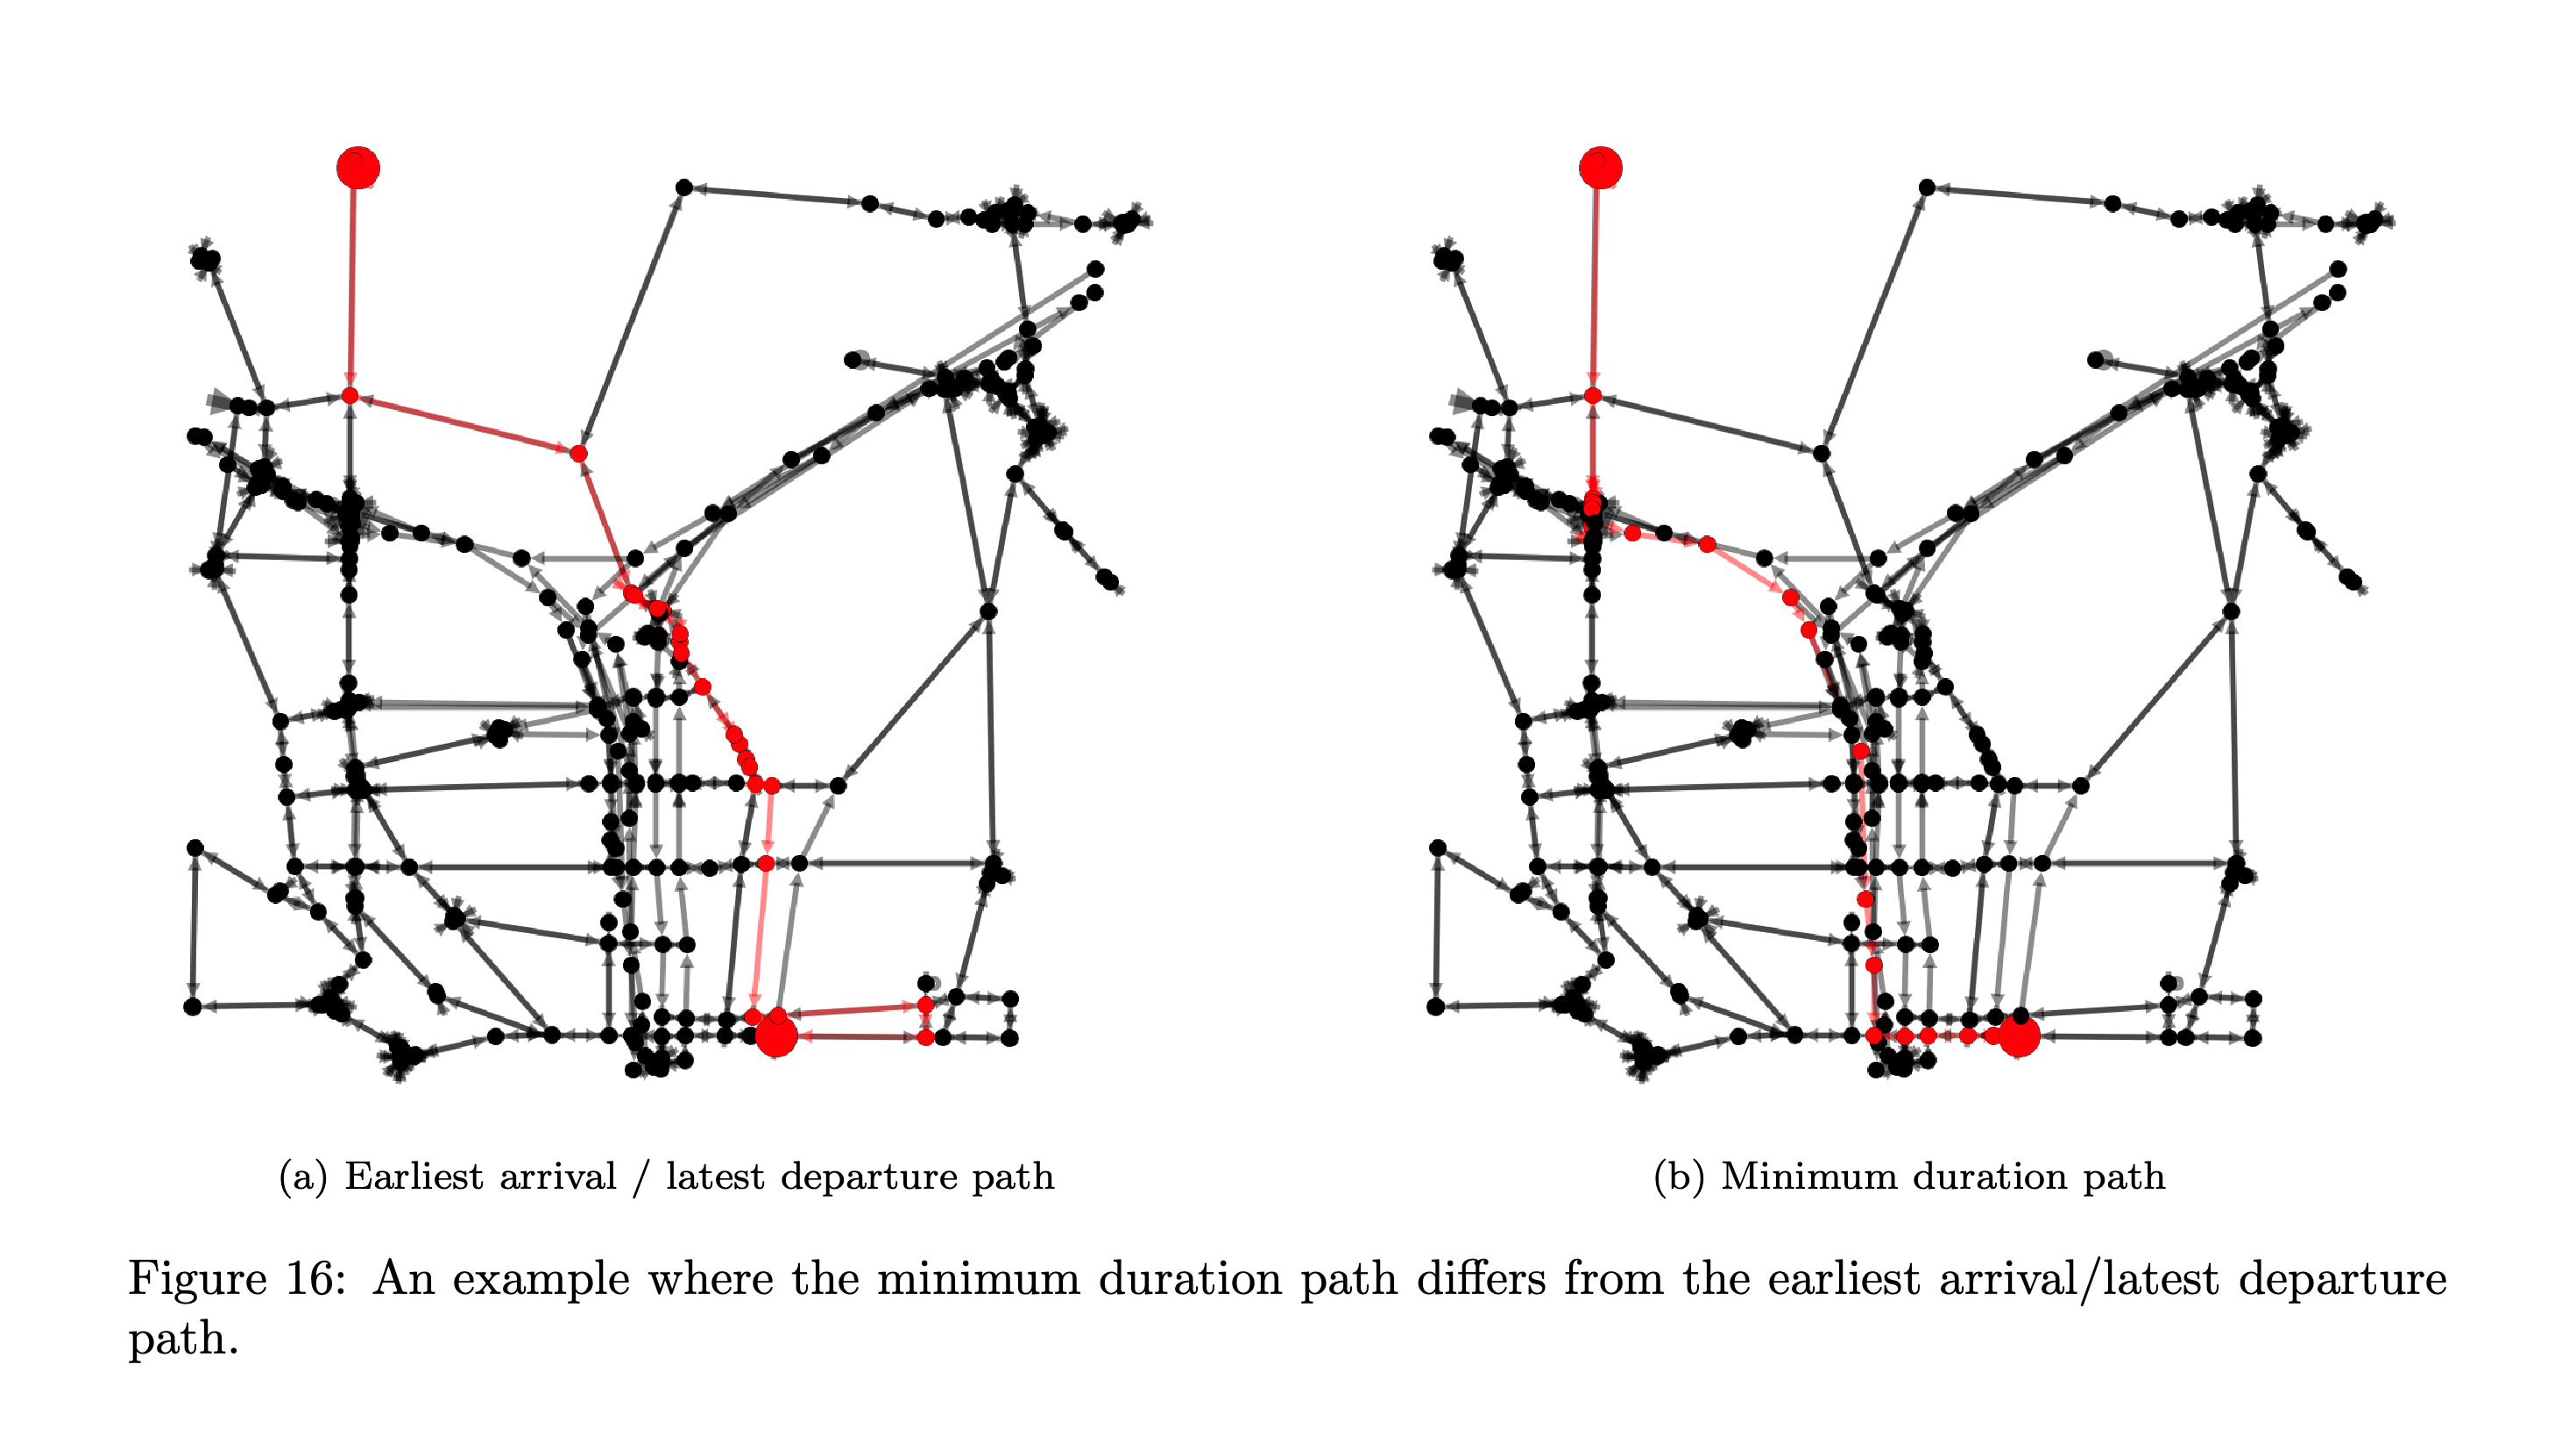
\includegraphics{images/Figure16.png} 

\begin{figure}
    \centering
    % \begin{subfigure}{0.45\textwidth}
        % \centering
    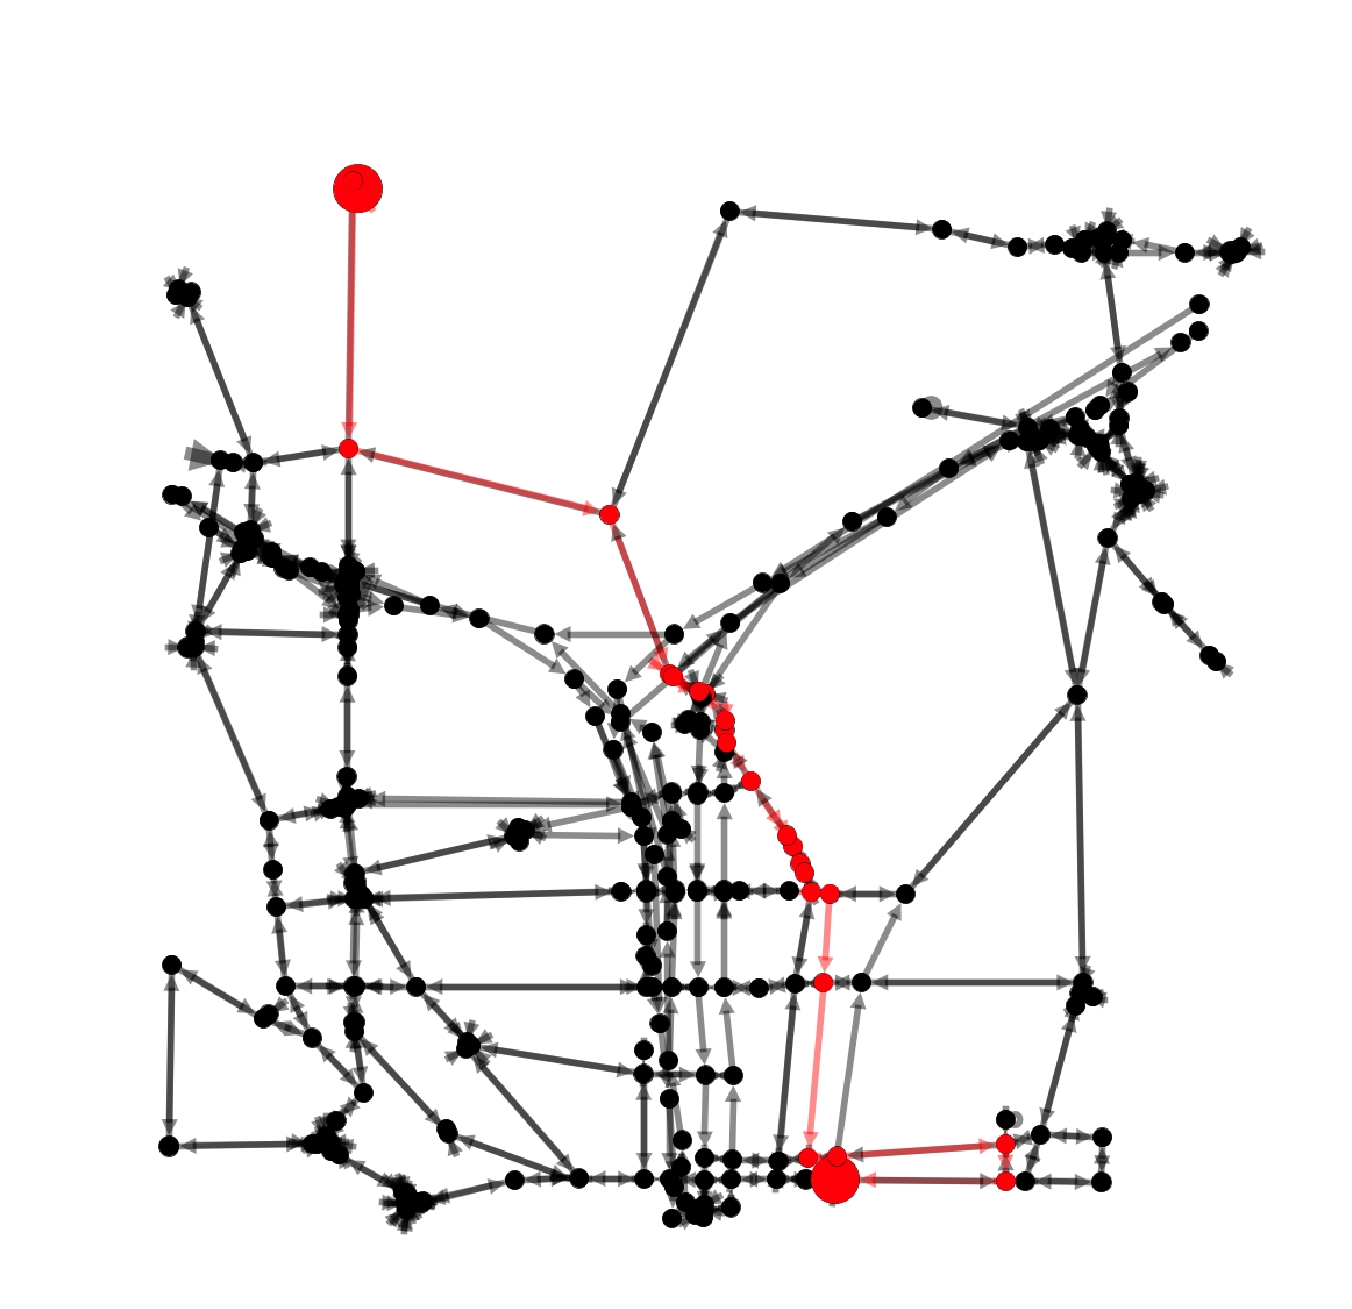
\includegraphics{edited-images/Figure16a.jpg}
        % \caption{}
        % \label{fig:16a}
    % \end{subfigure}
    % \begin{subfigure}{0.45\textwidth}
    %     \centering
    %     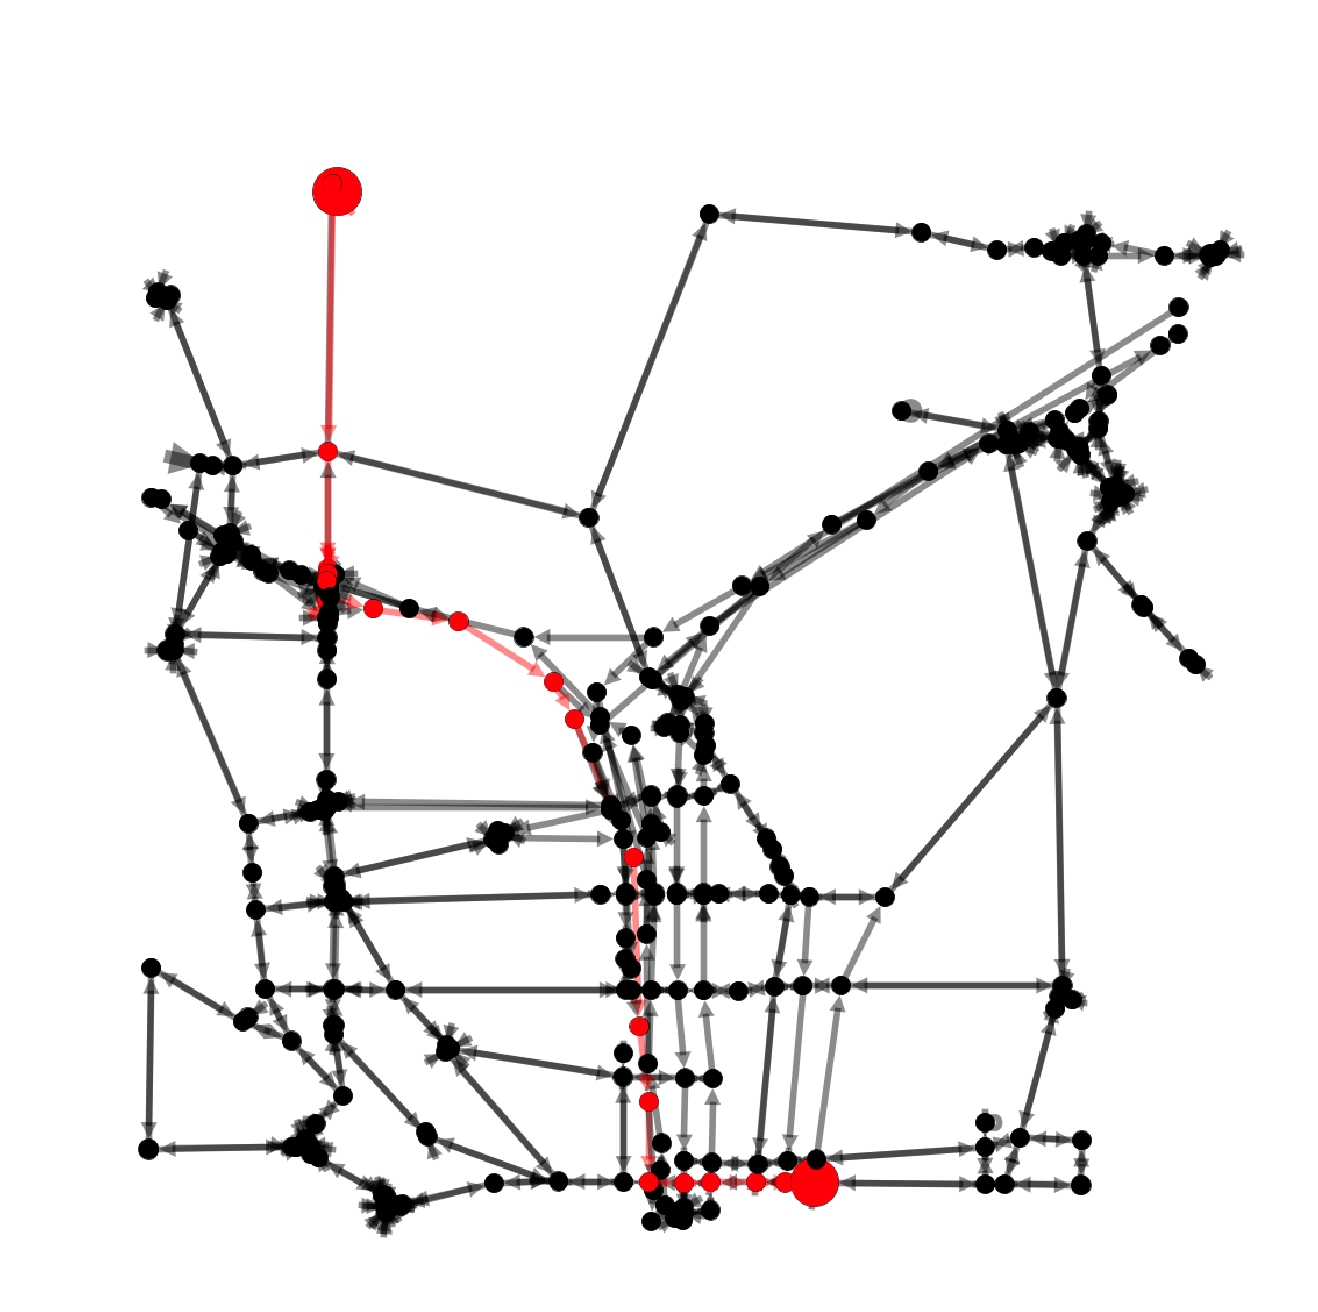
\includegraphics{edited-images/Figure16b.jpg}
    %     \caption{Thời gian thực hiện tối thiểu}
    %     \label{fig:16b}
    % \end{subfigure}
    \caption{Đường đi từ Bắc Atlanta đến Trung tâm Atlanta, đến đích sớm nhất / khởi hành muộn nhất}
    \label{fig:16}
\end{figure}
\backmatter
\end{document}
% END DOCUMENT